\section{LLMs-based Methods}
\subsection{Instruction Learning}
\begin{frame}
	\frametitle{Instruction Building}
	\begin{small}
	Instruction Building 是利用 LLMs 创建数据集的阶段。\\ 
	WizardLM 使用了 Evol-Instruct 方法让 LLM 自动生成高质量的 Instructions.
	\end{small}
	\begin{columns}
		\begin{column}{.2\textwidth}
			Evol-Instruct 从广度、深度、增加约束条件、具象化等方面演化。
		\end{column}
		\begin{column}{.8\textwidth}
	\begin{figure}[h]
		% \vspace{-2mm}
		\begin{center}
			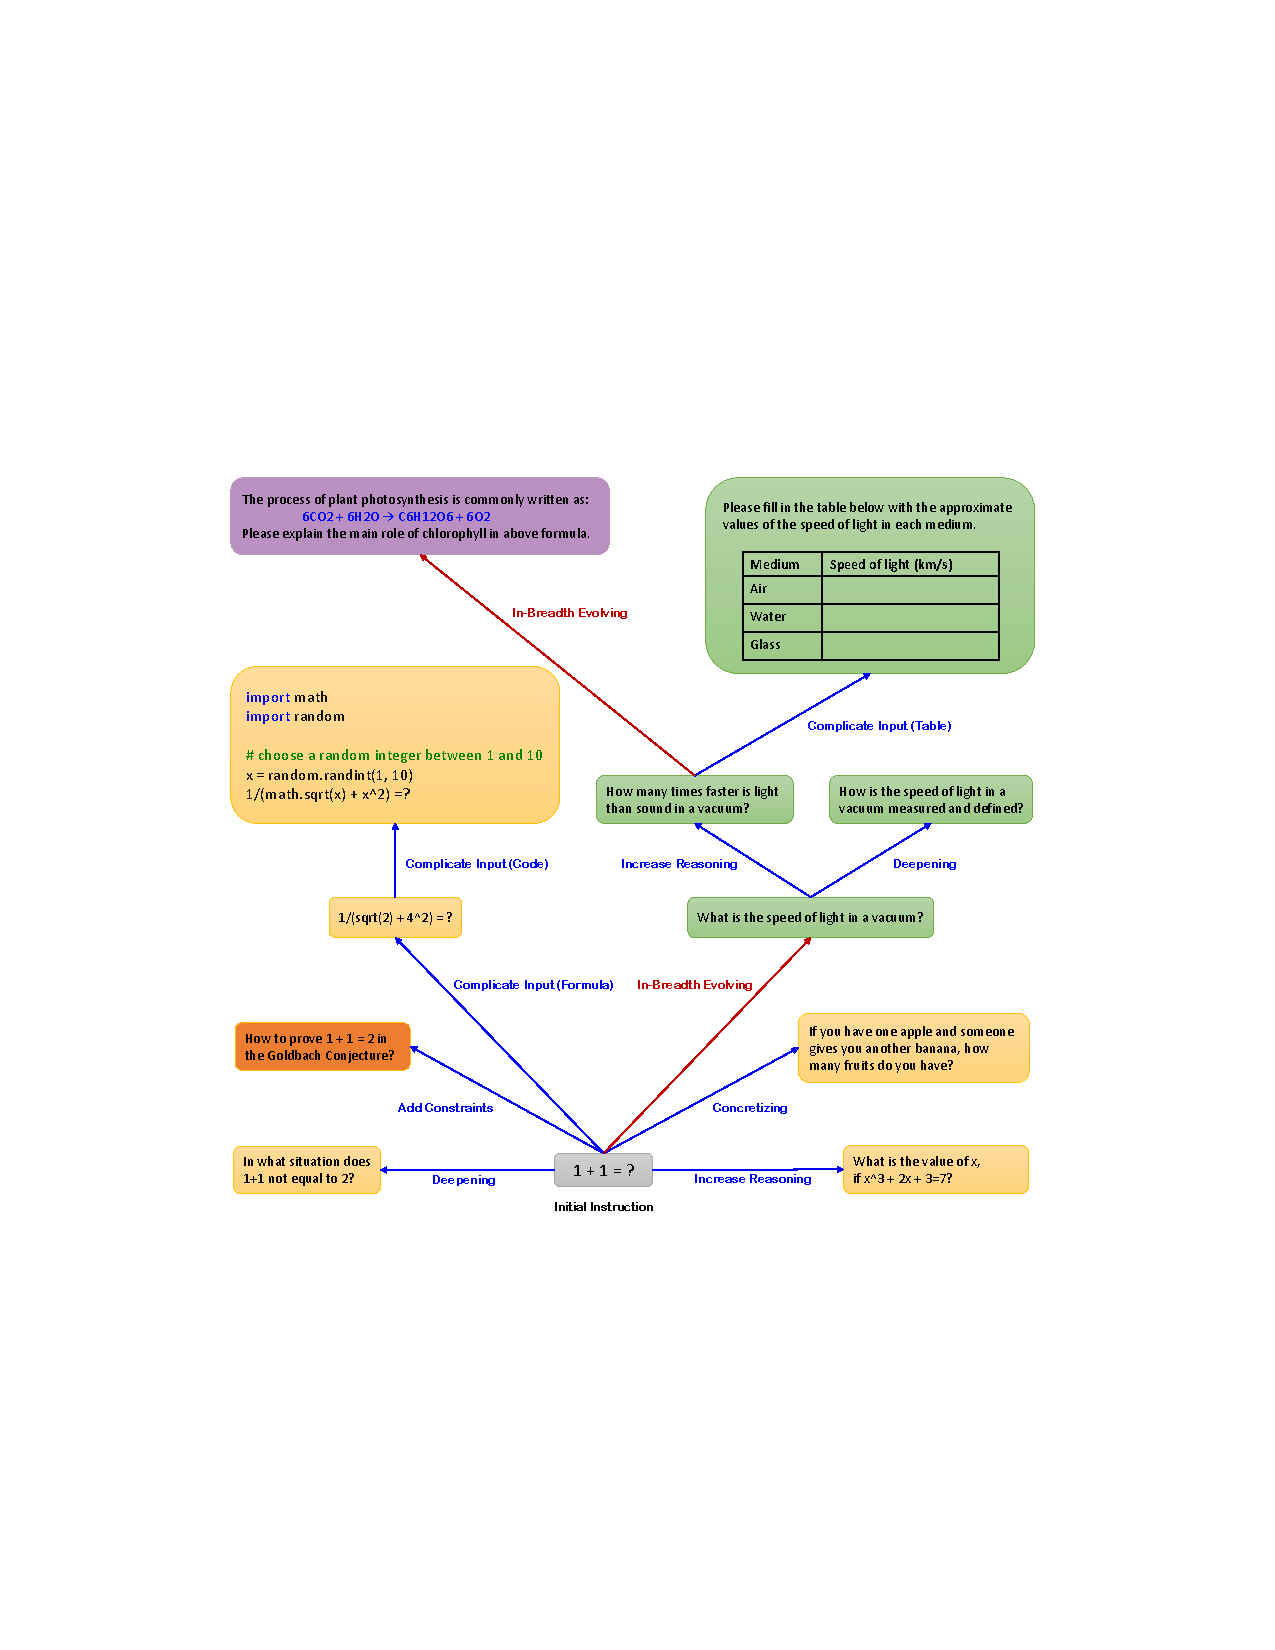
\includegraphics[width=0.5\textwidth]{pic/WizardLM.pdf}
		\end{center}
		\caption{Example of Evol-Instruct taken from WizardLM}
		\label{Evol-Instruct}
	\end{figure}
\end{column}
\end{columns}
\end{frame}

\begin{frame}
	\frametitle{Reinforcement Learning from Evol-Instruct
		Feedback (RLEIF)}
		\begin{columns}
			\begin{column}{.2\textwidth}
				{\small RLEIF 在 Evol-Instruct 的基础之上增加了  Process-supervised Reward Model (PRM) 作为监督模型,在 proximal policy optimization (PPO) 阶段会综合考虑这两个 reward model 的得分。}
			\end{column}
			\begin{column}{.8\textwidth}
	\begin{figure}
		\centering
		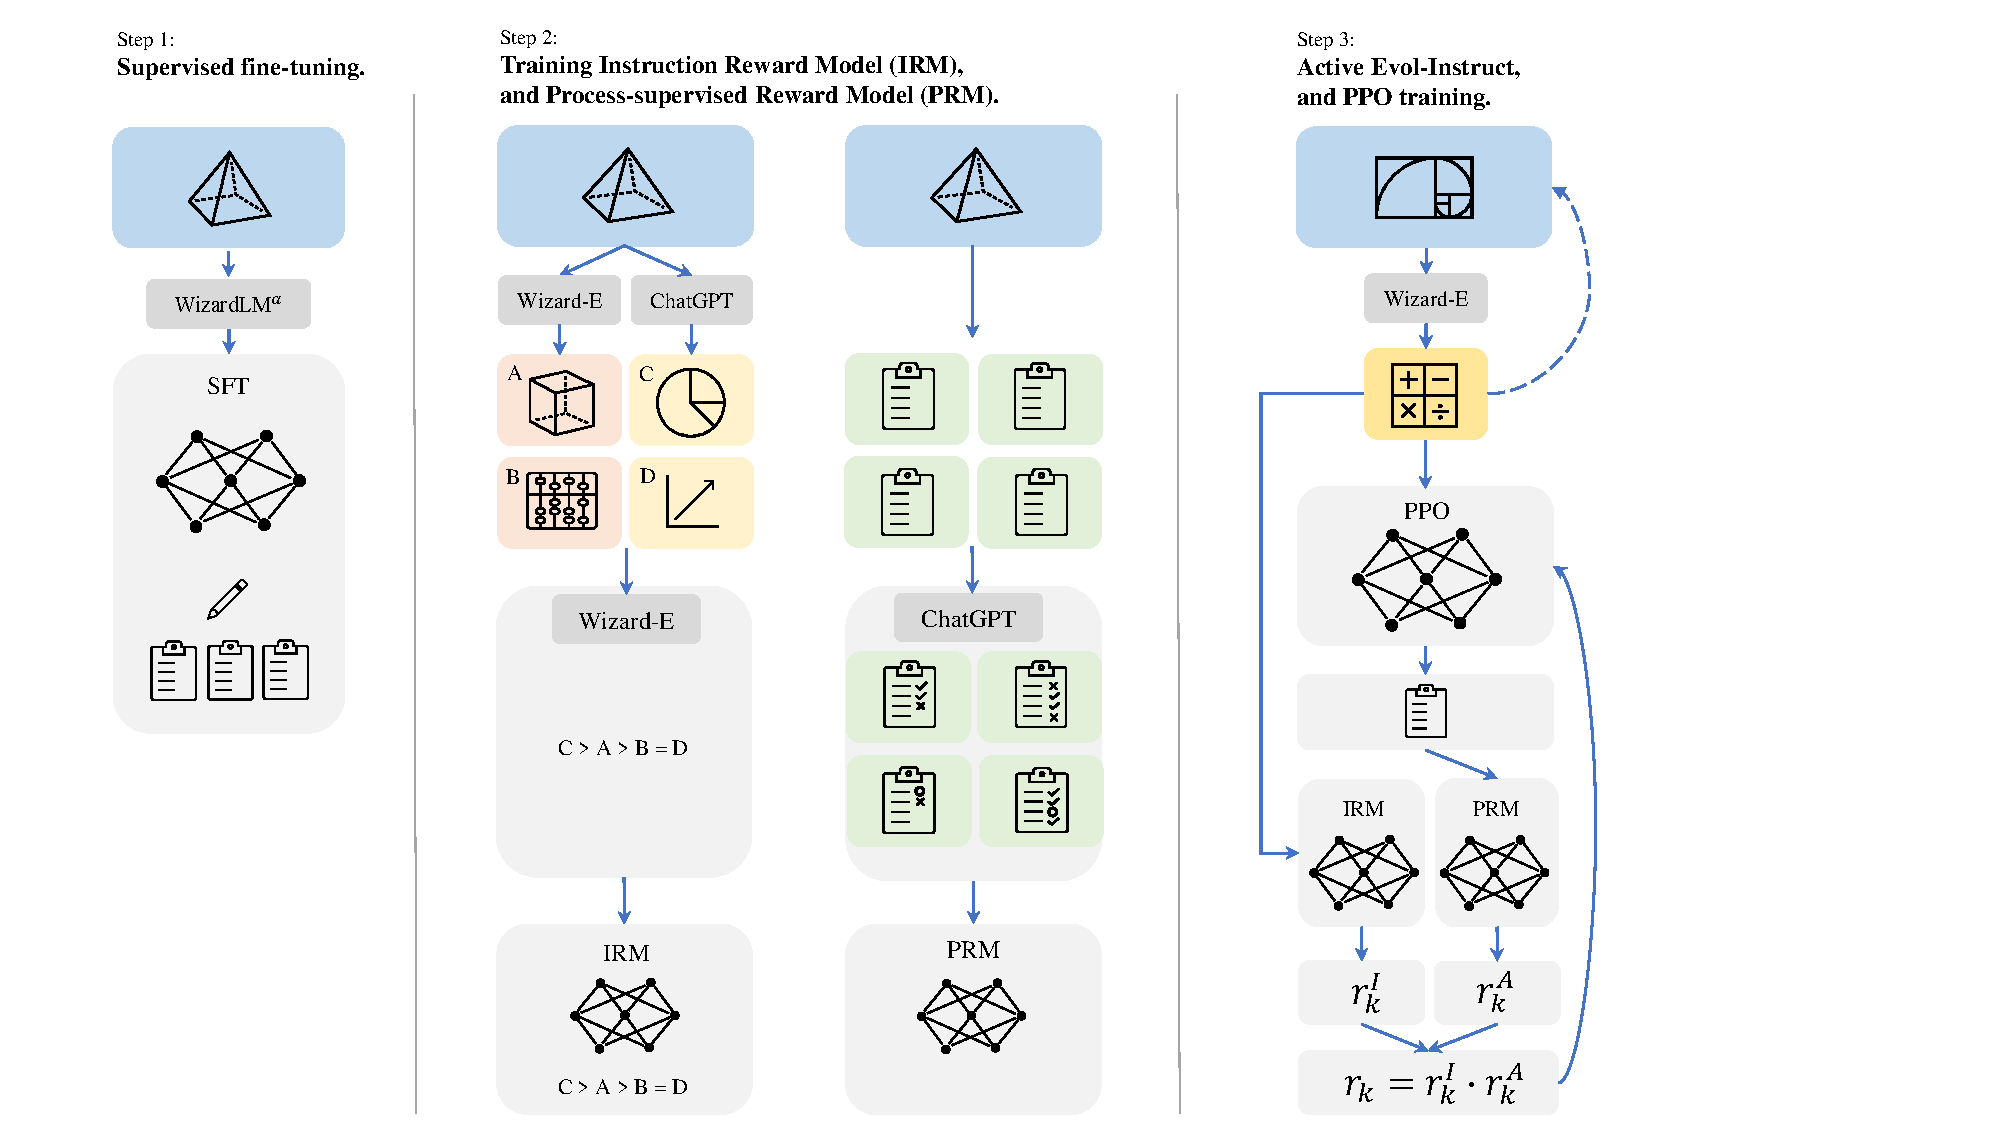
\includegraphics[width=0.7\textwidth, scale=1, trim=39 0 175 0,clip]{pic/reinforcement_evol_instruct.pdf}
		\caption{A diagram illustrating the three steps of RLEIF}
		\label{fig:reinforcement_evol_instruct_pic}
	\end{figure}
\end{column}
\end{columns}
\end{frame}

\begin{frame}
	\frametitle{Instruction Tuning}
	\textbf{PaLM 2-L-Math}:
	\begin{itemize}
		\item 发现 step-by-step 对于解题的质量提升有明显的效果。
		\item 综合使用 solution re-ranking 与 majority voting 会比单独使用效果更好。
		\item 通过多任务微调的方法,将生成解答和评估解答这两个任务分开,可以获得比只对解答进行单一微调更好的效果。
	\end{itemize}
\end{frame}

\begin{frame}
	\frametitle{In-context Learning (ICL)}
	ICL 是指通过在推理时提供特定任务示例,而无需更新模型参数。
	\begin{itemize}
		\item \textbf{ScratchpadGPT:}要求模型在 Scratchpad 中输出中间计算步骤,提升了正确率。
		\pause 
		\item \textbf{Codex-math:}通过生成代码的方式结合少样本学习自动生成解决数学问题的代码。
		\pause
		\item 选择复杂且多样化的示例可以提升推理性能。
	\end{itemize}
\end{frame}